\documentclass{suturo}
\usepackage{caption}
\usepackage{titlesec}
\begin{document}

\newcommand\tab[1][1cm]{\hspace*{#1}}

\titleformat{\paragraph}
{\normalfont\normalsize\bfseries}{\theparagraph}{1em}{}
\titlespacing*{\paragraph}
{0pt}{3.25ex plus 1ex minus .2ex}{1.5ex plus .2ex}

\makeatletter
\newcommand{\chapterauthor}[1]{%
  {\parindent0pt\vspace*{-27pt}%
  \linespread{0}\small\begin{flushright}von: #1\end{flushright}%
  \par\nobreak\vspace*{0pt}}
  \@afterheading%
}
\makeatother

\newpage
\section{Motion}
\subsection*{Zielsetzung}
\chapterauthor{Maximilian Bertram}
Das Ziel des Team Motion für den zweiten Meilenstein war es einen Actionserver zu implementieren, der verschiedene Aktionen für das Greifen, Abstellen und Umstoßen von Objekten anbietet. Jede der Aktionen soll mit jedem der vorhandenen Grippern möglich sein, dabei soll der Roboter Objekte in seiner Umgebung berücksichtigen und seine Bewegungspfade so planen, dass keine Kollisionen entstehen. Ist eine kollisionsfreie Bewegung nicht möglich wird die Aktion mit einem entsprechenden Fehler abgebrochen.\\
Ein weiteres Ziel waren genauere Rückgaben über den Erfolg der Aktionen, damit Knowledge seinen Beliefstate aktuell halten kann.\\

\subsection*{Probleme}
\chapterauthor{Maximilian Bertram, Roman Haak}
\subsubsection*{Kollisionsfreiheit beim Greifen eines Objektes}
Es war schwierig beim Greifen die kollisionsfreiheit mit anderen, herumstehenden Objekten, die nicht zur \textit{Planningscene} gehören, zu garantieren.\\
\textbf{Lösung}: Wir haben uns dazu entschieden die Bewegung für das Greifen und Abstellen auf einer Höhe auszuführen, auf der sich kein anderes Objekt befindet. Zuerst wird der gewünschte Gripper auf die 'sichere' Höhe gefahren und über das Objekt gefahren. Dann wird der Gripper geöffnet, richtig orientiert und nur auf einer Koordinatenachse (in negative Z-Richtung von '\textit{base\_footprint}') bewegt und so \textit{über} das Objekt geschoben.\\

\subsubsection*{Unterschiede Simulation echter PR2}
Teilweise wurden Lösungen implementiert, die in der Simulation sehr gut funktionierten. Aber als sie dann auf dem echten Roboter ausprobiert wurden,
funktionierten sie auf einmal nicht mehr.\\
\textbf{Lösung}: Leider gab es bei diesem Problem keine eindeutige Lösung. Lösungen mussten umgeschrieben werden, bis sie auch auf dem echten Roboter funktionierten.

\subsubsection*{'Deterministisches' Umstoßen eines Objektes}
Zunächst wurde das Umstoßen eines Objektes einfach dadurch realisiert, dass der Arm zu einem Punkt zwischen Roboter und Objekt gefahren wurde und danach zu dem Objekt. Dabei war es aber immer unterschiedlich, welchen Weg \textit{MoveIt} für die zweite Bewegung des Armes, also das Umstoßen, berechnet und ausgeführt hat.\\
\textbf{Lösung}: Die Funktion wurde so umgeschrieben, dass erst zu einem 'Zwischenpunkt' gefahren wird. Dann wird von diesem 'Zwischenpunkt' bis zu dem Punkt, an den der Gripper als zweites gefahren werden soll, eine 10-Punkte-Trajektorie berechnet. Diese Trajektorie beschreibt dann den geraden Weg von dem 'Zwischenpunkt' zum 'Umstoßpunkt' am Objekt. Und somit ist sichergestellt, dass immer von vorne umgestoßen wird.

\subsubsection*{Synchronisierung \textit{refactoren} des Codes und Implementierung}
Wir haben in einem \textit{branch} unseres Repositories angefangen zu \textit{refactoren}. In dem \textit{master-branch} wurde inzwischen weiterentwickelt. So kam es zu dem Problem, dass im master-branch stetig neue Funktionen hinzukamen, bzw. verändert wurden, welche dann in dem \textit{refactor-branch} wieder 'eingepflegt' werden mussten. Dadurch hat sich das \textit{refactoren} des Codes leider etwas in die Länge gezogen.\\
\textbf{Lösung}: Werden neue Funktionen eingebaut, werden diese direkt in den refactorten branch eingebaut, sodass dadurch kein Zusatzaufwand entsteht. Absprache ist in jedem Fall sehr wichtig.


\subsection{Übersicht des Teilsystems}
\chapterauthor{Roman Haak}
Die Untergruppe '\textit{Motion}' ist für das Bewegen verschiedener "Körperpartien" des Roboters zuständig.\\
Dabei wurde das Fahren des Roboters bis zu dem jetzigen Meilenstein von der Untergruppe '\textit{Planning}' übernommen, wird
in Zukunft aber von '\textit{Motion}' übernommen.\\
Das Bewegen der anderen, zum Erfüllen der Zielsetzung des Meilensteins 2 benötigten, Teile des Roboters, also Arm und Endeffektor (\textit{Gripper}) wurden 
von der Gruppe '\textit{Motion}' übernommen.\\

In \textit{Abbildung 1} Bild sieht man die Architektur des Teilsystems der Gruppe '\textit{Motion}'. Dabei gibt zwei Knoten '\textit{suturo\_motion\_main}' und '\textit{simple\_gripper}'.\\

\begin{figure}[!htb]
        \center{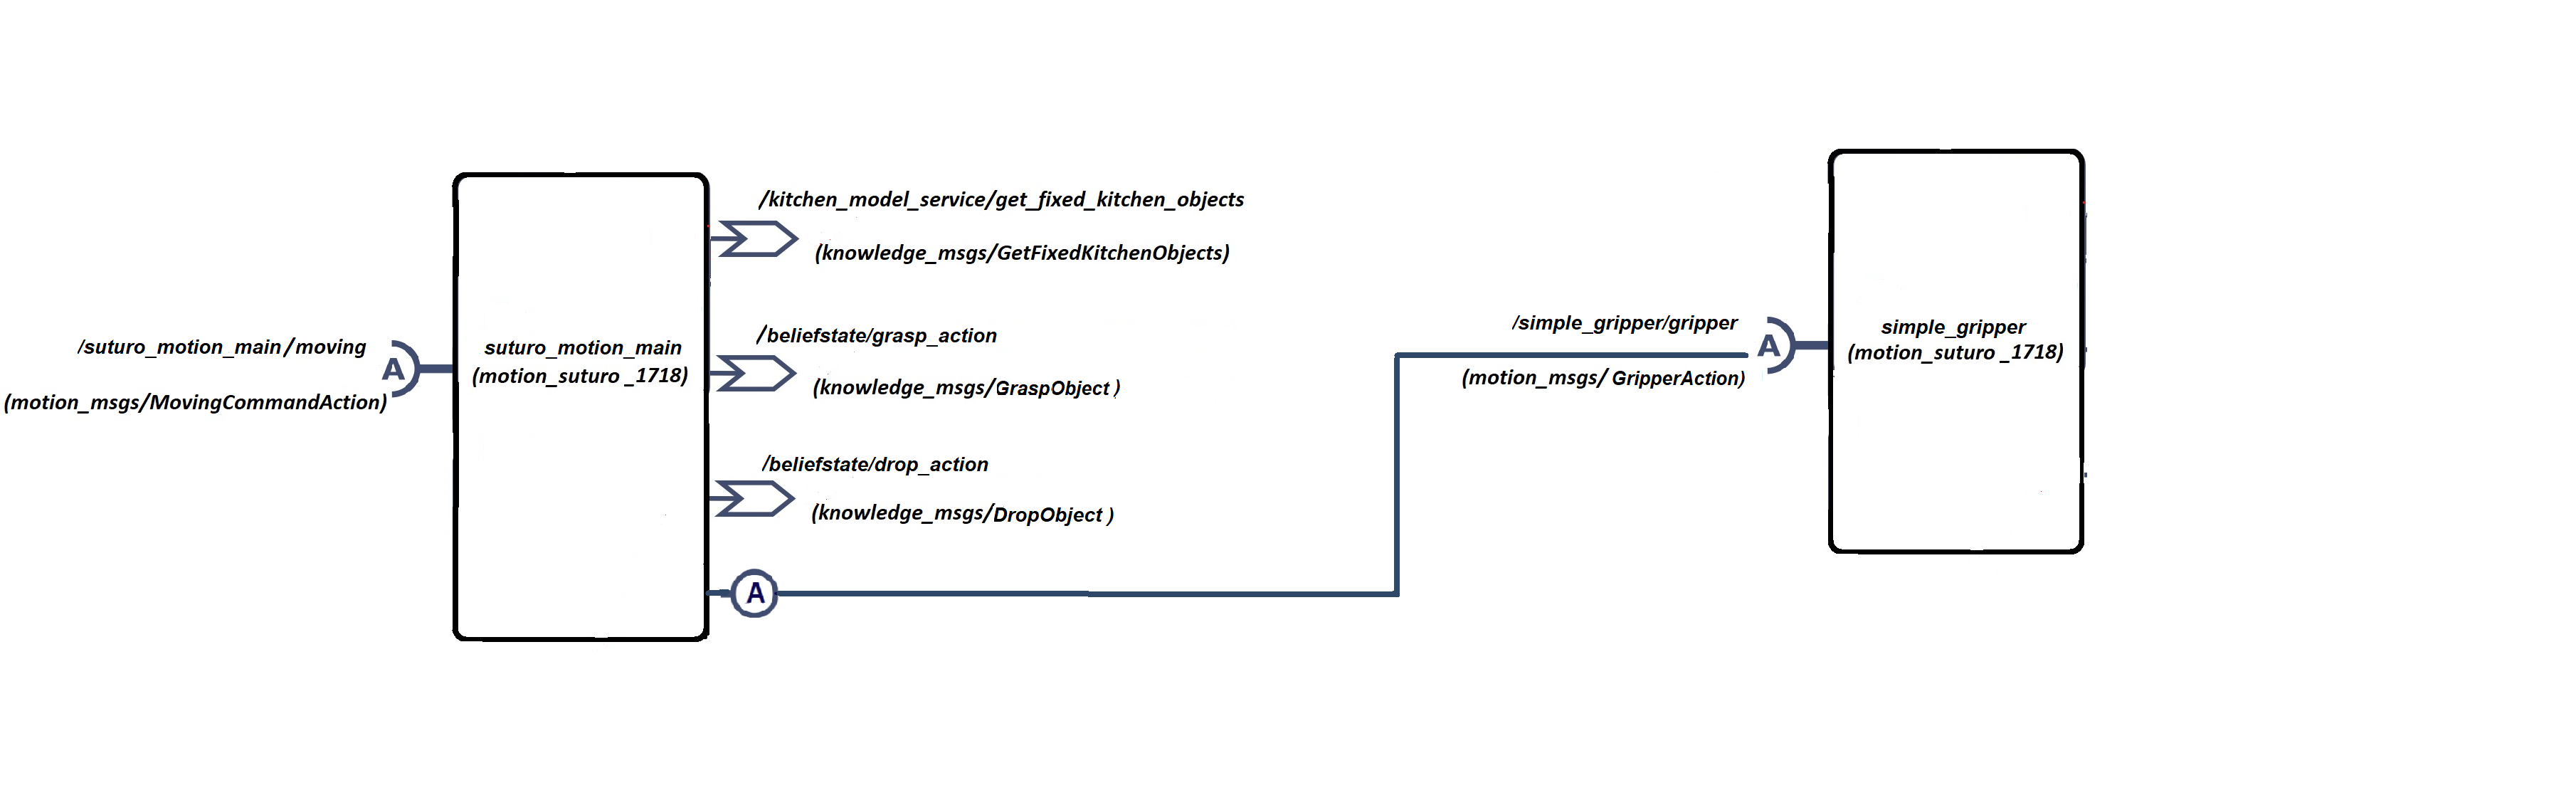
\includegraphics[width=\textwidth]
        {img/Architekturbild.png}
        \caption{\label{fig:motion_node} Architektur des Teilsystems der Gruppe 'Motion'}}
\end{figure}

Der Knoten '\textit{suturo\_motion\_main}' ist für das Verarbeiten eingehender Kommandos zum Bewegen der Arme bzw. eines Endeffektors zuständig. Dabei gibt es Kommandos für das Fahren der Arme in eine initiale Position, das Bewegen der Arme zu einer bestimmten Pose und das Umstubsen, Greifen oder Abstellen eines bestimmten Objektes mit einer bestimmten Pose.\\
Der Knoten '\textit{simple\_gripper}' wird dabei benutzt, um das Öffnen und Schließen des Endeffektors zu realisieren. Dieser Knoten wird von dem Hauptknoten '\textit{suturo\_motion\_main}' über einen Actionserver aufgerufen.\\

Im Folgenden werden die \textit{Schnittstellen}, der \textit{Ablauf} des Teilsystems, besonders \textit{hervorzuhebende} \textit{Algorithmen} und eine \textit{Installationsanleitung} beschrieben.\\

\subsection{Schnittstellen - 'suturo\_motion\_main'}
\subsubsection{Angebotene Actions}
\textbf{MovingCommand}
\chapterauthor{Maximilian Bertram}
Vom Typ '\textit{motion\_msgs/MovingCommand}': \\
\begin{lstlisting}[caption={Definition des MovingCommands},captionpos=b]
#goal definition
geometry_msgs/PoseStamped goal_pose
uint8 command
#constants for the command
uint8 UNKNOWN=0
uint8 MOVE_STANDARD_POSE=1
uint8 MOVE_RIGHT_ARM=2
uint8 MOVE_LEFT_ARM=3
uint8 POKE_RIGHT_ARM=4
uint8 POKE_LEFT_ARM=5
uint8 GRASP_RIGHT_ARM=6
uint8 GRASP_LEFT_ARM=7
uint8 PLACE_RIGHT_ARM=8
uint8 PLACE_LEFT_ARM=9
#Label of object which shell be grasped.
#Required because when an object gets grasped by robot,
#a message gets published from subgroup 'motion', which object
#has been grasped with which gripper (left or right).
#When the object gets placed somewhere, another message is published.
#These messages get published for knowledge's beliefstate, so that
#the knowledge component knows when an object get's grasped/placed somewhere.
string grasped_object_label
---
#result definition
bool successful
uint8 status
#constants for the status
uint8 SUCCESS=0
uint8 OUT_OF_RANGE=1
uint8 COLLISION=2
uint8 UNMANAGEBLE_ERROR=3
---
#feedback definition
#bool finished
\end{lstlisting}

Mit Hilfe der MovingCommandAction lassen sich alle von uns zur Verfügung gestellten Funktionen aufrufen. Es wurden Konstanten definiert, die die jeweilige Aktion beschreiben und in der Message-Definition vorhanden sind.

\subsubsection{Aufgerufene Actions}
Wird eine GRASP oder PLACE Aktion ausgeführt, wird über eine \\
\textit{pr2\_ controllers\_ msgs::Pr2GripperCommandAction} Message der Gripper entsprechend geöffnet oder geschlossen.\\
Dies ist nur eine Momentaufnahme, eigentlich sollte der Gripper über den Knoten '\textit{simple\_gripper}' geöffnet und geschloßen werden können (Siehe \textit{Abschnitt 1.3.1}),
aber es gab leider noch kleinere Probleme, weshalb wir das Öffnen/Schließen vorläufig über den direkten Weg realisieren.\\


\subsubsection{Aufgerufene Services}
\chapterauthor{RH, MB}
\textbf{GetFixedKitchenObjects}\\
Vom Typ '\textit{knowledge\_msgs/GetFixedKitchenObjects}': \\ 
\begin{lstlisting}[caption={Definition des GetFixedKitchenObjects-Service},captionpos=b]
// This servicedefinition is for transfering the shape of the objects in the iai_kitchen.
// The Motion-component calls this service for getting the shape of the kitchen-objects for it's planningscene.
// The Knowledge-component reads these shapes out of an owl-file and returns the data described below.


---
// The frame in which the object-poses are given.
string frame_id
// The names of the objects.
string[] names
// The bounding_boxes boxes of the objects.
geometry_msgs/Vector3[] bounding_boxes
// The poses of the objects.
geometry_msgs/Pose[] poses
\end{lstlisting}

\subsubsection{Benutzte Topics}
\textbf{GraspAction und DropAction}

Wird ein Objekt erfolgreich abgestellt oder gegriffen werden für den \textit{Beliefstate} von \textit{Knowledge} noch die entsprechenden \textit{Messages} gepublished: \\

\begin{lstlisting}[caption={Definition der GraspObject.msg},captionpos=b]
#A message which get's published by Motion-component after grasping an object.
#The label of the grasped object.
string object_label
#The gripper used. See 'Gripper.msg' for more details.
Gripper gripper
\end{lstlisting}

\begin{lstlisting}[caption={Definition der DropObject.msg},captionpos=b]
#A message which get's published by Motion-component after dropping an object.
#The gripper used. See 'Gripper.msg' for more details.
Gripper gripper
\end{lstlisting}

\begin{lstlisting}[caption={Definition der Gripper.msg},captionpos=b]
#A message for defining constants for differencing between left and right gripper.
uint8 gripper
#constants for gripper
uint8 LEFT_GRIPPER = 1
uint8 RIGHT_GRIPPER = 2
\end{lstlisting}

\subsection{Schnittstellen - 'simple\_gripper'}
\subsubsection{Angebotene Actions}
Vom Typ '\textit{motion\_msgs/Gripper}': \\
\begin{lstlisting}[caption={Definition der GripperAction},captionpos=b]
#goal definition
#position of the space between the grippers in meters
float64 position
#force in newton (default =  20)
float64 effort
#which grpper to open/closed
uint8 gripper
#Constants for the gripper value
uint8 LEFT_GRIPPER=1
uint8 RIGHT_GRIPPER=2
---
#result definition
bool successful
---
#feedback definition
#bool finished
\end{lstlisting}
\subsubsection{Aufgerufene Actions}
Die GripperAction-Message wird entsprechend geparsed und eine \\
 \textit{pr2\_ controllers\_ msgs::Pr2GripperCommandAction} erzeugt und gepublished. \\

\subsection{Ablauf}
\chapterauthor{Maximilian Bertram}
\subsubsection*{Schritt 1: Abfragen und hinzufügen der PlanningScene}
Beim Start der Node wird die PlanningScene (in unserem Fall die iai-Küche) bei Knowledge abgefragt und der MoveIt PlanningScene hinzugefügt.

\subsubsection*{Schritt 2: Parsen der Message}
Wird eine MovingCommandAction Message empfangen, wird diese zunächst geparsed. Je nachdem welche Konstante für das command feld gesetzt wird, wird die entsprechende Funktion des zugehörigen Controllers aufgerufen.

\subsubsection*{Schritt 3: Umrechnen der Pose}
Falls die Pose der Message in einem anderen Frame als dem PlanningFrame der zu bewegenden 
MoveGroup definiert wurde, wird die Pose mithilfe von TF in das PlanningFrame der zu bewegenden Gruppe transformiert.

\subsubsection*{Schritt 4: Planen der Bewegung}
Zunächst wird die Bewegung mithilfe des MoveIt Frameworks geplant. Ist die Bewegung nicht möglich, weil der Roboter die gewünschte Pose nicht erreichen kann oder es zu einer Kollision während der Bewegung kommen würde, wird die Aktion hier mit einer entsprechenden Fehlermeldung abgebrochen.

\subsubsection*{Schritt 5: Publishen von VisualizationMarkern}
Es werden VisualizationMarker gepublished um den Endpunkt der Bewegung in RViz zu visualisieren. Diese dienen hauptsächlich dem Debugging.

\subsubsection*{Schritt 6: Durchführen der Bewegung}
Ist die Bewegung kollisionsfrei möglich und die Pose erreichbar, wird die Bewegung durchgeführt und eine entsprechende Erfolgsmeldung zurückgegeben.

\subsubsection*{Schritt 7: Rückmeldung an Knowledge Service}
Falls es sich um ein \textit{GRASP} oder \textit{PLACE} Aktion handelt und die Aktion erfolgreich war wird der Knowledge Service aufgerufen um den Beliefstate zu aktualisieren. Es wird übergeben, welches Objekt sich in welchem Gripper befindet.


\subsection{Besonderheiten/Besondere Algorithmen}
\chapterauthor{Roman Haak}
In diesem Abschnitt werden kurz erwähnenswerte Algorithmen beschrieben.
Dabei wird zuerst der Algorithmus für das Umstoßen eines Objektes und anschließend der Algorithmus für das Greifen, bzw. Abstellen eines Objektes beschrieben.\\

\subsubsection{Algorithmus für das Umstoßen eines Objektes}
Über die von unserem Teilsystem angebotene Action '\textit{moving}' kann das Kommando zum Umstoßen eines Objektes mit dem rechten oder mit dem linken \textit{Gripper} abgesetzt werden. Beim Aufruf wird dabei eine Pose übergeben, welche die Position des Mittelpunktes des umzustoßenden Objektes und die beabsichtigte Orientierung des \textit{Grippers} beinhaltet. \\Der Algorithmus, der das Umstoßen dann realisiert, arbeitet wie folgt:\\

1. \textit{Berechne die Pose, zu der der Arm als erstes gefahren werden soll. Diese Pose wird folgendermaßen ermittelt:}\\
\tab - die Orientierung wird von der beim Aufruf des Kommandos übergebenen Pose übernommen\\
\tab - die Position ist die Position des Objektmittelpunkts, von der noch die Distanz\\ \tab   'DISTANCE\_BEFORE\_POKING' und 'GRIPPER\_LENGTH\_LEFT'\\ \tab bzw. 'GRIPPER\_LENGTH\_RIGHT' von der X-Koordinate im 'base\_footprint'-Frame \\ \tab abgezogen wird, wobei 'DISTANCE\_BEFORE\_POKING', 'GRIPPER\_LENGTH\_LEFT' \tab und 'GRIPPER\_LENGTH\_RIGHT' definierte Konstanten sind.\\

Der so errechnete Zielpunkt befindet sich also 'DISTANCE\_BEFORE\_POKING' plus 'GRIPPER\_LENGTH\_LEFT' bzw. 'GRIPPER\_LENGTH\_RIGHT' vor dem Objekt, aus Sicht des Roboters.\\

2. \textit{Fahre mit dem rechten bzw. linken Arm zu der errechneten Pose.}\\

3. \textit{Errechne nun einen Punkt, der etwas über dem Objektmittelpunkt liegt und falls der linke Arm benutzt wird, noch um 'GRIPPER\_LENGTH\_LEFT' minus 'GRIPPER\_LENGTH\_RIGHT' näher am Roboter liegt, damit immer auf dieselbe Weise umgestoßen wird, egal ob der linke (längere) oder rechte Arm benutzt wird.}\\

4. \textit{Berrechne eine 10-Punkte Trajektorie zwischen dem in Schritt 3 errechneten Punkt und der aktuellen Position des Armes.}\\
\tab - Dies hat den Sinn, dass sichergestellt ist, dass das Objekt von\\ \tab vorne umgestoßen wird.\\

5. \textit{Fahre den Arm entlang der gewünschten Trajektorie.}\\
\tab - Das Objekt sollte nun umgestoßen worden sein.


\subsubsection{Algorithmus für das Greifen/Abstellen eines Objektes}
Über die von unserem Teilsystem angebotene Action '\textit{moving}' kann das Kommando zum Greifen/Abstellen eines Objektes mit dem rechten oder mit dem linken \textit{Gripper} abgesetzt werden. Beim Aufruf wird dabei eine Pose übergeben, welche die Position des Greifpunktes des zu greifenden Objektes, bzw. die Position, zu der der \textit{Gripper} hingefahren werden soll, um das Objekt abzustellen beinhaltet. Zusätzlich ist noch die beabsichtigte Orientierung des \textit{Grippers} beinhaltet. \\Der Algorithmus, der das Greifen bzw. Abstellen dann realisiert, ist dabei derselbe. Denn die beiden Aktionen Greifen und Abstellen unterscheiden sich bei uns momentan nur daran, dass beim Greifen der \textit{Gripper} erst geöffnet und dann zum Greifen geschloßen wird und beim Abstellen der \textit{Gripper} zuerst bereits geschloßen ist und beim Abstellen des Objektes dann geöffnet werden muss. Zu dieser Unterscheidung reichen also Fallunterscheidungen innerhalb des Algorithmus. \\Der Algorithmus arbeitet dabei wie folgt:\\

1. \textit{Hebe den gewünschten Arm auf die Höhe 'TABLE\_HEIGHT' + 'MAXIMUM\_OBJECT\_HEIGHT' + 'GRIPPER\_LENGTH\_LEFT' + 'DISTANCE\_BEFORE\_GRASPING'.}\\
\tab - Da wir es in unserem aktuellen Stand des Gesamtsystems noch nicht geschafft haben, \\ \tab beim Greifen die Kollisionsfreiheit sicherzustellen, haben wir uns entschieden das Greifen\\ \tab aus einer Höhe zu realisieren, auf der sich sicher kein Objekt befindet.\\

2. \textit{Bewege den Arm auf dieser Höhe über das zu greifende/abzustellende Objekt.}\\

3. \textit{Ändere die Orientierung des Armes zu der Orientierung, die in der übergebenen Pose beinhaltet ist.}\\
\tab - Die übergebene Orientierung ist in dem aktuellen Stand die, bei der der \textit{Gripper} nach \\ \tab unten orientiert ist, damit das Objekt so gegriffen werden kann.\\

4. \textit{Hier findet eine Fallunterscheidung statt.}\\
\tab - Soll ein Objekt gegriffen werden, öffne den \textit{Gripper}.\\
\tab - Soll ein Objekt abgestellt werden, lass den \textit{Gripper}, wie er ist.\\

5. \textit{Fahre mit dem Arm zu der in der übergebenen Pose angegebenen Position.}\\

6. \textit{Hier findet wieder eine Fallunterscheidung statt.}\\
\tab - Soll ein Objekt gegriffen werden, schließe den \textit{Gripper}.\\
\tab - Soll ein Objekt abgestellt werden, öffne den \textit{Gripper}.\\

7. \textit{Hebe den Arm wieder auf die am Anfang errechnete Höhe an, um das Objekt zu heben, bzw. "vom Objekt wegzufahren".}\\
\tab - Das Objekt sollte nun entweder an dem gewünschten Platz stehen, bzw. sich in dem\\ \tab \textit{Gripper} des Roboters befinden.


\subsection{Tests \& Evaluation}
\chapterauthor{MB, RH}
Da wir agil entwickeln, haben wir abgewägt und die Priorität auf die Zielerreichung des 2.
Meilensteines gesetzt und uns gegen das Implementieren von Unit-Tests durch ein Testframework entschieden. Alle von Motion angebotenen Funktionen (greifen, abstellen, umstubsen) wurden mehrfach manuell am echten Roboter überprüft und getestet. Die Implementierung von Unit-Tests wird im 3. Meilenstein folgen. \\

Durch die händischen Tests sind immer wieder Differenzen zwischen echtem PR2 und der Simulation aufgefallen. Es mussten immer wieder Anpassungen am Code vorgenommen werden, damit das Package auf dem jeweiligen System wie gewünscht funktioniert. Die Fehlersuche hat hierbei enorm Zeit verbraucht. \\

Am Ende funktionierten die angebotenen Funktionalitäten wie gewünscht, jedoch mit kleineren Fehlern/Unschönheiten.\\

\subsection{Installationsanleitung}
\chapterauthor{Maximilian Bertram}

\begin{itemize}
\item[a] Zunächst müssen folgende Repositories in den source-Ordner des Workspaces hinzugefügt werden:  \\
\url{https://github.com/menanuni/motion_suturo_1718} \\
\url{https://github.com/menanuni/msgs_suturo_1718} \\
\url{https://github.com/menanuni/knowledge_suturo_1718} \\

\item[b] Es muss das MoveIt Framework installiert werden, dazu im Terminal: \\
\textit{sudo apt-get update} \\
\textit{sudo apt-get install ros-indigo-moveit} \\
\textit{echo  \grqq{}source /opt/ros/indigo/setup.bash\grqq{} \textgreater\textgreater \textasciitilde{ }/.bashrc} \\

\item[c] Jetzt kann das System über \textit{catkin build} gebaut werden.
\end{itemize}

Den Stand der für Stand  des 2. Meilensteins findet sich unter folgendem Tag: \\
-TODO: LINK TAG-

\subsection{Starten der Nodes}
\chapterauthor{Roman Haak}
\begin{itemize}

\item Soll das System im Kontext des echten Roboters benutzt werden, muss zunächst über \textit{roslaunch kitchen\_model\_export knowledge\_export\_service.launch} ein Teilsystem von \textit{Knowledge} gestartet werden.

\item Unser Teilsystem wird über \textit{roslaunch motion motion\_main\_start.launch} gestartet werden, falls er im Kontext einer Simulation ausgeführt werden soll, bzw. \textit{roslaunch motion motion\_main\_start\_real\_pr2.launch}, falls der Knoten auf dem PR2 ausgeführt werden soll.

\item Dann können Befehle an den Actionserver unseres Knotens über das Topic \textit{/moving/goal} abgesetzt werden. Zur Erläuterung des Actionservers siehe Dokumentation der Gruppe \textit{motion}.
\end{itemize}


\end{document}
